\chapter{Generalised belief propagation}
\label{ch:gbp}

Chapter~\ref{ch:overlap} measured what $\mathrm{BP}_{\chi}$ loses to
non-trivial overlap. This chapter runs the repair the literature already has,
Kikuchi's in the message-passing form of \citet{yedidia2005} and
Sec.~\ref{sec:gbp-intro}, on the same three classes, and measures what it
recovers.

\begin{figure}[t]
\centering
\begin{adjustbox}{max width=\linewidth}
\begin{tikzpicture}
% ---- left: the graph, with its two complexes
\node[nd] (v0) at (-4.5,0) {};
\node[nd] (v1) at (-3.55,0.6) {};
\node[nd] (v2) at (-3.55,-0.6) {};
\node[nd] (v3) at (-2.6,0) {};
\node[lb,anchor=east] at (-4.62,0) {$0$};
\node[lb,anchor=south] at (-3.55,0.72) {$1$};
\node[lb,anchor=north] at (-3.55,-0.72) {$2$};
\node[lb,anchor=west] at (-2.48,0) {$3$};
\draw[lnk] (v0)--(v1) (v0)--(v2) (v1)--(v2) (v1)--(v3) (v2)--(v3);
\begin{scope}[on background layer]
  \node[cx,fit=(v0)(v1)(v2)] {};
  \node[cxb,fill opacity=0.72,fit=(v1)(v2)(v3)] {};
\end{scope}
\node[lb,anchor=north,align=center] at (-3.55,-1.35) {the two complexes};

\node[lb] at (-1.55,0) {$\Longrightarrow$};

% ---- right: the region graph they close on
\node[cxb,inner sep=3.2pt] (P1) at (0.2,1.0) {$\{0,1,2\}$};
\node[cxb,inner sep=3.2pt] (P2) at (3.1,1.0) {$\{1,2,3\}$};
\node[cx,inner sep=3.2pt]  (R)  at (1.65,-0.75) {$\{1,2\}$};
\node[lb,anchor=south] at (0.2,1.32) {$c=+1$};
\node[lb,anchor=south] at (3.1,1.32) {$c=+1$};
\node[lb,anchor=north] at (1.65,-1.07) {$c=-1$};
\draw[msg] (P1) -- node[lb,pos=0.52,xshift=-8.5mm] {$m_{P_{1}\to R}$} (R);
\draw[msg] (P2) -- node[lb,pos=0.52,xshift=8.5mm] {$m_{P_{2}\to R}$} (R);
\node[lb,anchor=north,align=center] at (1.65,-1.75)
  {the region graph, and the two messages on it};
\end{tikzpicture}
\end{adjustbox}
\caption{\textbf{What generalised belief propagation runs on.} Left: the two
complexes of Fig.~\ref{fig:sharededge}, meeting in the pair $\{1,2\}$. Right:
the family closed under intersection, with the counting numbers
Eq.~\eqref{eq:mobius} assigns. The shared pair is a region in its own right and
carries $c=-1$, so the bond inside it is counted $1+1-1=1$ time rather than
twice, which is the arithmetic the cavity method got wrong. A message runs from
each parent region to its child, Eq.~\eqref{eq:p2c}, and carries what the parent
knows about the child's two variables. Here the three regions form a junction
tree and the fixed point is exact; Secs.~\ref{sec:sixty} to~\ref{sec:realoverlap}
ask what happens when they do not.}
\label{fig:regiongraph}
\end{figure}

\section{Region graphs}
\label{sec:regions}
\index{region graph|textbf}
\index{junction tree|textbf}
\index{chordal graph|textbf}
\index{generalised belief propagation|textbf}
\index{Kikuchi approximation|textbf}

The repair is the next level of the same construction, available since
Kikuchi. Figure~\ref{fig:regiongraph} is it on the two triangles of
Chapter~\ref{ch:overlap}: the closed family, the counting number each region
carries, and where the messages run.

Belief propagation is exact on a tree because a tree can be decomposed into
nodes and edges with each variable counted once. When it is not a tree, the
remedy is to work with larger \emph{regions} --- sets of variables treated as
units --- and to choose counting numbers so that every variable, and every
interaction, is still counted once.

Close the complex family under intersection and assign counting numbers by
M\"obius inversion:
\begin{equation}
  c_{R}=1-\sum_{R'\supsetneq R}c_{R'}.
  \label{eq:mobius}
\end{equation}

Two things follow.

\emph{It contains what the book has been doing.} When complexes meet in at most
one node, the family closes on the complexes plus the single nodes, and
Eq.~\eqref{eq:mobius} gives $c_{v}=1-k$ --- precisely the counting of
Eq.~\eqref{eq:bethe}. Chapter~\ref{ch:statmech}'s free energy was a region-graph
free energy all along, on the region graph a treelike chygraph happens to have.
That is why Sec.~\ref{sec:freeenergy} could say its weights were not chosen.

\emph{It departs from it exactly where complexes overlap.} On two triangles
sharing an edge, M\"obius inversion puts $-1$ on the shared \emph{edge};
Eq.~\eqref{eq:bethe} puts $-1$ on each of its two endpoints. Both count every
node once. Only one counts the shared \emph{bond} once: summing the counting
numbers of every region containing $\{1,2\}$ gives $1$ under
Eq.~\eqref{eq:mobius} and $2$ under Eq.~\eqref{eq:bethe}. The Bethe scheme
subtracts the two shared vertices independently and so never removes the
correlation between them.

The example has four spins and can be settled by enumeration.


\section{Two triangles sharing an edge}
\label{sec:twotriangles}

Couple every pair inside each triangle --- the shared bond carrying one coupling
and not one per triangle, so that the object is the five-edge graph the two
triangles make --- evaluate $\ln Z$ exactly by summing over all sixteen
configurations, and compare (Table~\ref{tab:twotriangles}).

\begin{table}[t]
\centering\small
\begin{tabular}{rrrrr}
\hline\hline
$\beta J$ & exact & Bethe & M\"obius & GBP\\
\hline
$0.2$ & $2.8887$ & $+1.8\times10^{-2}$ & $-1.4\times10^{-3}$ & $-4\times10^{-14}$\\
$0.5$ & $3.5907$ & $+9.1\times10^{-2}$ & $-2.9\times10^{-2}$ & $-2\times10^{-13}$\\
$1.0$ & $5.7390$ & $+3.7\times10^{-1}$ & $-6.6\times10^{-2}$ & $-3\times10^{-14}$\\
$2.0$ & $10.6938$ & $+1.3$ & $-1.7\times10^{-2}$ & $-5\times10^{-15}$\\
\hline\hline
\end{tabular}
\caption{\textbf{Two triangles, by exact enumeration.} $\ln Z$ for the five-edge graph made by two triangles sharing a bond, against the error made by the Bethe counting, the M\"obius counting evaluated on isolated regions, and generalised belief propagation iterated to a fixed point on the region graph. The two countings err in opposite directions; running the messages removes the overshoot entirely. Computed in \code{figs/\allowbreak overlap.\allowbreak py}.}
\label{tab:twotriangles}
\end{table}

The correction is a factor of three to eighty, so the counting matters. The two
schemes err in \emph{opposite} directions:
Eq.~\eqref{eq:bethe} overestimates $\ln Z$ because it never removes the
correlation between the shared vertices, and Eq.~\eqref{eq:mobius} removes it
and slightly overshoots.

The overshoot is a property of evaluating a counting on \emph{isolated}
regions, which is an estimate rather than a fixed point, and not of the counting
itself. Running the messages removes it entirely. The last column is
generalised belief propagation in its parent-to-child form \citep{yedidia2005},
iterated to a fixed point on the region graph of Eq.~\eqref{eq:mobius}, and the
error is at the level of double precision at every coupling.

A message lives on a directed edge of the region graph, from a region $P$ to a
direct child $R$, and is a function of the child's variables. Write
$U_{R}=\{R\}\cup\mathrm{descendants}(R)$, and $f_{R}$ for the product of every
factor whose scope lies inside $R$. The belief on a region collects every
message entering $U_{R}$ from outside it,
\[
  b_{R}(x_{R})\ \propto\ f_{R}(x_{R})
    \!\!\prod_{(I\to J):\ J\in U_{R},\ I\notin U_{R}}\!\! m_{I\to J}(x_{J}),
\]
and imposing the consistency condition $\sum_{x_{P}\setminus x_{R}}b_{P}=b_{R}$
cancels every message common to the two sides. What is left is the update:
\begin{equation}
  m_{P\to R}(x_{R})=
  \frac{\displaystyle\sum_{x_{P}\setminus x_{R}}f_{P\setminus R}(x_{P})
        \prod_{N(P,R)}m}
       {\displaystyle\prod_{D(P,R)\setminus(P,R)}m},
  \label{eq:p2c}
\end{equation}
with
\[
  \begin{aligned}
    N(P,R)&=\{(I,J):J\in U_{P}\setminus U_{R},\ I\notin U_{P}\},\\
    D(P,R)&=\{(I,J):J\in U_{R},\ I\in U_{P}\setminus U_{R}\}.
  \end{aligned}
\]
The two index sets look forbidding and are doing something simple: $N$ collects
what flows into the part of $P$ that is not $R$, and $D$ divides out what has
already been counted on the way down.

The check that this is the right generalisation is what it degenerates to. On
the two-layer region graph of a pairwise model --- one region per interaction
plus one per variable --- $D(P,R)$ holds only the edge being updated, $N(P,R)$
is the set of incoming messages to the interaction's other variables, and
Eq.~\eqref{eq:p2c} \emph{is} ordinary belief propagation. So generalised belief
propagation contains belief propagation exactly as Eq.~\eqref{eq:mobius}
contains Eq.~\eqref{eq:bethe}, and Sec.~\ref{sec:overlap-checks} reports the
numerical form of that statement. \code{gbp.\allowbreak GBP} is Eq.~\eqref{eq:p2c} and \code{region.\allowbreak RegionGraph} the family it runs on.

The region family closes on $\{0,1,2\}$, $\{1,2,3\}$ and $\{1,2\}$ once the
zero-counting singletons are dropped, and that is a junction tree: a tree of
regions in which the intersection of any two regions is contained in every
region on the path between them. Generalised belief propagation on a junction
tree is exact, for the same reason belief propagation on a tree is.

So the whole of what the table reports as left on the table is recoverable ---
but by an argument that says exactly when it is recoverable, which is when the
closed complex family is a junction tree. For maximal cliques that means the
graph is chordal, and a hyperbolic random graph is not.

One more thing this calculation settles. Generalised belief propagation refuses
to run on a region graph whose counting numbers do not cover every factor once,
and the Bethe counting on two overlapping triangles is exactly such a graph. The
failure is detected rather than silently absorbed: the scheme knows the shape of
its own assumption. \code{region.\allowbreak RegionGraph} closes the family and reports whether it is a junction tree, which is the test the rest of the chapter turns on.

The rest of the chapter measures that comparison on three ensembles, chosen so
that the origin of the triangles differs while the clustering does not:
hyperbolic random graphs, where the triangles come from an underlying geometry
(Sec.~\ref{sec:sixty}); the Karrer--Newman ensemble, where they are placed by
hand (Sec.~\ref{sec:karrer}); and real networks, where they are whatever the
data recorded (Sec.~\ref{sec:realoverlap}). Section~\ref{sec:merging} then asks
what the alternative repair, merging, costs on the same three.


\section{Hyperbolic random graphs}
\label{sec:sixty}

Figure~\ref{fig:gbp} runs the three schemes over sixty maximal-clique region
graphs of hyperbolic random graphs at $n=14$, $18$ and $20$, small enough to
enumerate exactly, at mean degrees $3.5$, $5$ and $7$ and two couplings, keeping
only the instances that are not already treelike. Those sizes and densities are
the ones Secs.~\ref{sec:karrer} and~\ref{sec:realoverlap} match.

\begin{figure}[t]
\centering
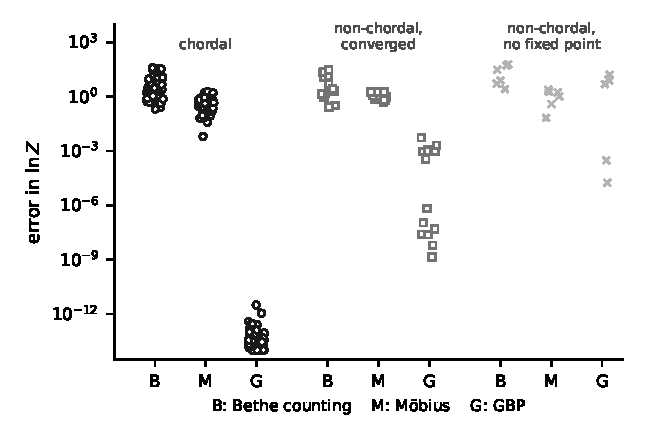
\includegraphics[width=\linewidth]{figs/fig-gbp.pdf}
\caption{\textbf{Hyperbolic random graphs.} Error in
$\ln Z$ for sixty maximal-clique region graphs of hyperbolic random graphs,
under the Bethe counting (B), the M\"obius counting evaluated on isolated
regions (M), and generalised belief propagation run to a fixed point (G).
Where the clique structure is chordal the region graph is a junction tree and
GBP is exact. Where it is not, GBP still gains two to nine orders of magnitude
--- when it converges. On six of the twenty non-chordal instances it does not
converge at all, even at damping $0.999$, and no number from them is quoted.
Data from
\code{statmech/\allowbreak probe/\allowbreak gbp\_\allowbreak cliques.\allowbreak py}; plotted by \code{figs/\allowbreak overlap.\allowbreak py}.}
\label{fig:gbp}
\end{figure}

The forty chordal instances come out exact, the worst error being
$3\times10^{-12}$: Sec.~\ref{sec:twotriangles}'s argument holding over sixty
instances.

The twenty non-chordal instances divide in two. Fourteen converge, and there the GBP error runs from
$1.4\times10^{-9}$ to $5.4\times10^{-3}$, against $0.48$ to $1.8$ for the
M\"obius counting and $0.26$ to $30$ for the Bethe counting on the same
instances --- two to nine orders of magnitude better, with the consistency
condition $\sum_{x_{P}\setminus x_{R}}b_{P}=b_{R}$ satisfied to
$2\times10^{-6}$, so what remains is the approximation's error and not the
solver's.

The other six do not converge, at any damping tried up to $0.999$. Their
residual says so, and no number from them is quoted.

\paragraph{Two limits.} Generalised belief propagation is not variationally bounded, so on a
region graph built from complexes that contain one another it can be
\emph{worse} than the static estimate --- covering $K_{4}$ by its four triangles
rather than by $K_{4}$ itself gives an error of $10^{-2}$ against a static
$4\times10^{-3}$. That particular case does not arise for maximal
cliques, which never nest --- but nesting is only one route to it.
Section~\ref{sec:realoverlap} finds sound fixed points on maximal-clique region
graphs, no nesting anywhere among them, that are still worse than the static
estimate. What non-nesting removes is one mechanism, not the absence of the
guarantee, and either way it is a reason not to build region graphs carelessly.

And it is an \emph{instance-level} calculation. It takes an explicit list of
complexes and an explicit interaction. Everything else in this book works at the
level of an ensemble, where a message is a distribution over a chy-degree class
rather than a function on one region.


\section{The Karrer--Newman ensemble}
\label{sec:karrer}
\index{Karrer--Newman model|textbf}
\index{null model}

The second ensemble places its triangles rather than growing them
(Sec.~\ref{sec:threeclasses}). Because two placed motifs share an edge only by
coincidence, it is treelike above the level of the motif by construction, and
the question is what that buys the messages.


\paragraph{The enumeration ceiling falls inside the crossover.}
Sections~\ref{sec:sixty} and~\ref{sec:realoverlap} enumerate $\ln Z$ exactly,
which caps the instances at twenty vertices. On this ensemble that cap is not a
mild restriction, because the property that defines it is asymptotic. The number
of triangle pairs sharing an edge is $O(1)$ while the number of cliques grows
like $n$, so the fraction of cliques caught in an overlap falls like $1/n$ ---
and at twenty vertices it has not begun to fall (Table~\ref{tab:knfinite}).

\begin{table}[t]
\centering\small
\begin{tabular}{rrrr}
\hline\hline
$n$ & offending pairs & per clique & treelike\\
\hline
$14$ & $10.7$ & $0.84$ & $0$\%\\
$20$ & $19.2$ & $0.87$ & $0$\%\\
$50$ & $35.4$ & $0.58$ & $0$\%\\
$100$ & $38.6$ & $0.32$ & $0$\%\\
$500$ & $57.5$ & $0.098$ & $0$\%\\
$2000$ & $58.6$ & $0.025$ & $0$\%\\
\hline\hline
\end{tabular}
\caption{\textbf{The placed ensemble at small $n$.} Maximal-clique pairs sharing
two or more atoms, and that count divided by the number of cliques, for
Karrer--Newman graphs at $\ave{k}=5$; mean over twelve seeds. The count
saturates, as the $O(1/n)$ coincidence argument requires. The per-clique rate
falls like $1/n$, from $0.84$ at the enumeration ceiling to $0.025$ at
$n=2000$ --- a factor of thirty-four. No sample at any size was treelike.
Generated by \code{figs/\allowbreak merge.\allowbreak py:check\_\allowbreak placed\_\allowbreak finite\_\allowbreak size}.}
\label{tab:knfinite}
\end{table}

At $n\le20$ every sample drawn was non-treelike and five sixths of its cliques
were caught in an overlap. Whatever the messages do there, they are not doing it
on the ensemble Sec.~\ref{sec:merging} will measure; they are doing it on a
small dense graph that happens to have been generated by placing triangles.

\paragraph{What the messages buy here.} Sixty runs on thirty instances, ten at
each of $n=14$, $18$ and $20$ with realised mean degrees $2.9$, $3.9$ and $5.4$.
Every one of the thirty graphs drawn was non-treelike, at every size, so the
filter that discards treelike instances discarded nothing.

Only two of the sixty runs are chordal, against $40$ of $60$ on the hyperbolic
ensemble and $56$ of $120$ on the real neighbourhoods. The placed ensemble is
the \emph{least} chordal of the three at these sizes, which inverts what its
defining property would lead one to expect and is the direct consequence of
Table~\ref{tab:knfinite}: at twenty vertices its triangles overlap almost
everywhere.

Of the $58$ non-chordal runs, $43$ reach a fixed point that is both converged
and consistent --- and here, unlike the real neighbourhoods, the two tests never
disagree: every run that reached a residual below $10^{-9}$ also had consistent
beliefs. On those $43$ the GBP error runs from $5\times10^{-3}$ to $1.9$ against
$2.6\times10^{-2}$ to $6.2$ for the M\"obius counting on the same instances.

That is a gain of $-0.1$ to $1.7$ orders of magnitude, with a median of $0.3$.
On the hyperbolic ensemble the same comparison gave two to nine orders. Running
the messages on this ensemble at these sizes buys a factor of two in the error
and not a factor of a thousand, and on one instance --- $n=20$, the strongest
overlap in the sample, at a consistency of $8\times10^{-16}$ --- it lands
$+1.018$ from the exact answer where the static counting it was meant to improve
is at $-0.876$.

The sizes are also where the iteration starts to fail: at $n=14$ and $18$,
$18$ of $20$ runs reach a sound fixed point; at $n=20$, seven do.

These are not measurements of the Karrer--Newman ensemble but of what the
messages do on small dense graphs generated by placing triangles;
Table~\ref{tab:knfinite} is the distinction. What the ensemble does at its own
scale is Sec.~\ref{sec:coretransition}'s question.



\section{Real networks}
\label{sec:realoverlap}
\index{overlap!in real networks}

The same three schemes run on the six real networks of
Sec.~\ref{sec:threeclasses}, in their two families.
Figure~\ref{fig:gbpreal} reports them.

Twenty vertices is the enumeration ceiling, so the instances are
\emph{neighbourhoods} rather than whole networks: a vertex with its neighbours,
induced, kept when it has between eight and twenty vertices and its maximal
cliques are not already treelike. Overlap between complexes is local --- two
complexes meeting in two atoms --- and a vertex's neighbourhood is where it
occurs.



\begin{figure}[t]
\centering
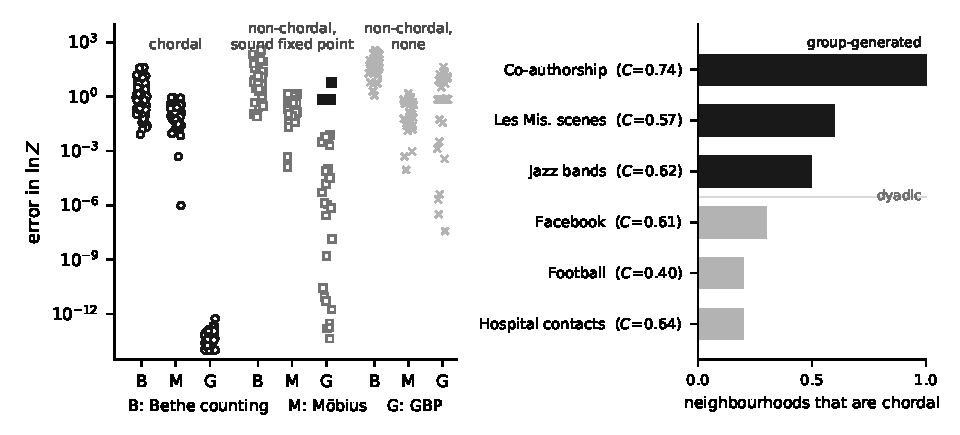
\includegraphics[width=\linewidth]{figs/fig-gbp-real.pdf}
\caption{\textbf{Real networks.} Left: the three schemes
of Fig.~\ref{fig:gbp} over 120 runs on 60 maximal-clique region graphs, taken as
induced neighbourhoods of six real networks at two couplings. A fixed point
counts as sound when the messages have stopped moving \emph{and} the beliefs
agree where they overlap; on hyperbolic graphs the two conditions never came
apart, and here they do. Filled squares are the four sound fixed points that
came out no better than the static M\"obius estimate they were to improve.
Right: the fraction of each network's neighbourhoods that are chordal, and so
exactly solved for free. The split follows how the edges were recorded, not the
clustering coefficient $C$ beside each name --- the two families overlap in $C$
and in neighbourhood density alike. Data from \code{statmech/\allowbreak probe/\allowbreak gbp\_\allowbreak real.\allowbreak py}; plotted
by \code{figs/\allowbreak overlap.\allowbreak py}.}
\label{fig:gbpreal}
\end{figure}

\paragraph{Chordality follows provenance, not clustering.} Of the
group-generated neighbourhoods $21$ of $30$ are
chordal; of the dyadic ones $7$ of $30$. Since a chordal clique family is a
junction tree, that is the fraction on which the repair is exact and costs
nothing, and the $56$ chordal runs come out exact to $5\times10^{-13}$.

The two families do not differ in the obvious ways. Their clustering
coefficients overlap --- $0.57$ to $0.74$
against $0.40$ to $0.64$ --- and so do the densities of the neighbourhoods
themselves, $0.46$ to $0.72$ against $0.49$ to $0.80$. The most clustered
network in the study is the co-authorship one at $C=0.74$, and every one of its
neighbourhoods is chordal; the second most clustered is hospital contact at
$C=0.64$, and two of ten are. Les Mis\'erables at $C=0.57$ in the sparser
neighbourhoods gets $6$ of $10$, hospital contact at $C=0.64$ in the denser ones
gets $2$. More clustering does not mean more chordal, and denser does not mean
less; where the cliques came from does.

Take a vertex whose neighbourhood is generated by groups, and let the groups it
belongs to be $A_{1},\dots,A_{k}$, each a clique. The induced neighbourhood is
their union. If the $A_{i}$ pairwise meet only in the vertex itself the family is
treelike and this chapter has nothing to say about it; those are filtered out. If
they meet in more, the union is still a union of cliques glued along shared
sets, and such a graph is chordal unless the \emph{pattern of intersections}
itself carries a cycle --- three groups meeting pairwise in different pairs of
members, with no single group containing all of them. That is a much stronger
demand than a chordless four-cycle, which is all it takes to spoil chordality in
general.

A dyadic neighbourhood has no such protection. Its maximal cliques are not
primitive objects that something placed; they are whatever the triangles happen
to assemble into, and four vertices joined in a ring with neither diagonal
present is the generic case rather than a conspiracy.

The chygraph mapping is therefore best behaved where the data supplies its
complexes and worst where they must be inferred from dyads, which is
Chapter~\ref{ch:data}'s statement about $\bar s$ from the other direction. The chordality fractions behind the claim are counted in \code{statmech/\allowbreak probe/\allowbreak gbp\_\allowbreak real.\allowbreak py}, one neighbourhood at a time.

\paragraph{A small residual stops certifying an answer.} Of the $64$ non-chordal runs, $38$ drive the residual below $10^{-9}$.
On the hyperbolic instances every converged run also satisfied
$\sum_{x_{P}\setminus x_{R}}b_{P}=b_{R}$ to $2\times10^{-6}$. Here $8$ of the
$38$ stop moving without the beliefs agreeing, by margins as large as
$6\times10^{-2}$: the messages reach a state they do not leave, and it is not a
fixed point of the variational problem. Those runs are set aside; the $30$ that
pass both tests are what the rest of this section quotes.

That the second test is doing real work, and is not a formality the first
already covers, has an independent check. The whole measurement was run twice,
same instances and same protocol, differing only in the floating-point summation
order that comes of scheduling the work differently. The $86$ runs that pass
both tests reproduce to $2\times10^{-12}$ in $\ln Z$. The $8$ that reach a small
residual without consistent beliefs do not reproduce at all: the largest
disagreement between the two runs is $14.19$ in $\ln Z$, on a hospital-contact
neighbourhood that reached a residual of $10^{-12}$ both times and landed
$-22.08$ from the exact answer once and $-7.88$ the other. A state that is not a
fixed point of the variational problem is not a quantity, and the residual alone
does not distinguish the two.

\paragraph{Where the messages lose to the static estimate.} On the
group-generated side the sound fixed points behave as in Fig.~\ref{fig:gbp}:
$12$ of them, error from $4\times10^{-14}$ to $1\times10^{-4}$, four
to thirteen orders of magnitude below the static M\"obius counting, and not one
worse than it. On the dyadic side there are $18$, the error runs to $5.9$, the
gain runs from $9$ orders \emph{down to} $-1.5$, and four of the eighteen are no
better than the static estimate they were meant to improve.

Three of the four are at the stronger coupling and two of those sit at
$-\ln 2$ to six decimal places --- the signature of a fixed point that has
selected one of the two spin-reversed states and lost the other from $Z$. That
is a recognisable mode and arguably the solver's fault rather than the
approximation's. The fourth is not accounted for that way. On an eleven-vertex
neighbourhood of the football network, with eighteen maximal cliques and no
nesting anywhere among them, the messages reach a residual of
$8\times10^{-13}$ and a consistency of $3\times10^{-15}$ --- as clean a fixed
point as anything in the chordal column --- and land $5.85$ away from the exact
$\ln Z$, where the static M\"obius counting is off by $0.63$. Its beliefs are
ordered where the exact model is not, carrying a mean $|m|$ of $0.85$ at a
coupling of $0.3$ against zero by spin-reversal symmetry; but one state selected
out of two accounts for $\ln 2=0.69$ of the deficit and leaves the other $5.16$
unexplained. Nine times the static error, with nothing in the convergence to
indicate it.

\section{What the chapter settles}
\label{sec:gbpverdict}

Generalised belief propagation is exact when the closed region family is a
junction tree, which for maximal cliques means the graph is chordal. That holds
on $98$ of the $240$ runs, and on those the error is at most
$3\times10^{-12}$.

On the other $142$ it is not. Figure~\ref{fig:gbpvsbp} puts both calculations on
the axis of Fig.~\ref{fig:cavityfail}. The chordal runs lie along the bottom at
machine precision. The rest scatter between $10^{-11}$ and $10^{1}$, below
$\mathrm{BP}_{\chi}$ but not near zero, and the two do not track: over the
non-chordal runs the correlation between the two logarithms is $-0.22$.

\begin{figure}[t]
\centering
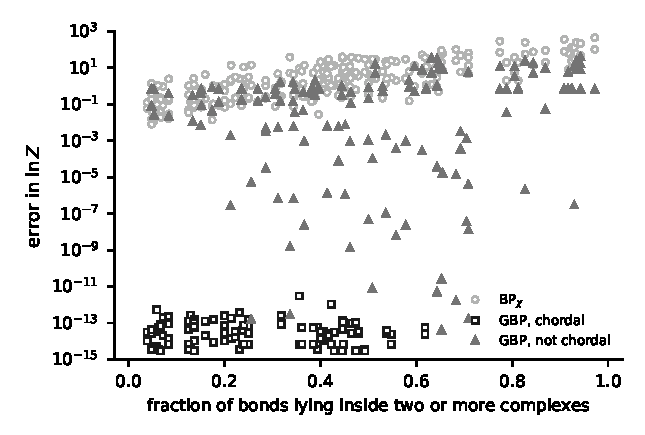
\includegraphics[width=\linewidth]{figs/fig-gbp-vs-bp.pdf}
\caption{\textbf{GBP against $\mathrm{BP}_{\chi}$.} Error in $\ln Z$ for
$\mathrm{BP}_{\chi}$ and for generalised belief propagation on the same $240$
runs, against the axis of Fig.~\ref{fig:cavityfail}. GBP is exact on the chordal
instances and improves on $\mathrm{BP}_{\chi}$ nearly everywhere else --- median
$0.31$ against $2.73$ over the non-chordal runs --- while reaching exactness on
none of them. Generated by \code{figs/\allowbreak overlap.\allowbreak py}.}
\label{fig:gbpvsbp}
\end{figure}

So the scheme is not a weaker version of the cavity method: it is the better
number almost everywhere, by a factor of about nine on the median of the
non-chordal runs, and it is worse on $39$ of $142$. What it does not do is
remove the error. It reaches exactness only where the clique family is already a
junction tree --- which is to say where the chygraph's incidence structure is
already a tree, and the failure of Chapter~\ref{ch:overlap} was smallest to
begin with. Chapter~\ref{ch:metacomplex} takes the other route.


\section{Checks}
\label{sec:overlap-checks}

\checkhead{Known results}
The counting numbers of Eq.~\eqref{eq:mobius} and the parent-to-child update of
Eq.~\eqref{eq:p2c} are Kikuchi's and \citeauthor{yedidia2005}'s, and the
implementation is checked against them. On the two-layer region graph of a
pairwise model --- one region per interaction plus one per variable --- the
update reduces to ordinary belief propagation, and the implementation reproduces
an independently written one to $10^{-10}$ on a chain, a star, a four-cycle and
a theta graph. The loopy error is included, so the two agree on the mistake as
well as on the answer. That is the check that generalised belief propagation
contains belief propagation exactly as Eq.~\eqref{eq:mobius} contains
Eq.~\eqref{eq:bethe}.

\checkhead{New results}
What the messages recover, on three classes of network, is new. Where the
iteration converges on the hyperbolic instances the consistency condition
$\sum_{x_{P}\setminus x_{R}}b_{P}=b_{R}$ holds to $2\times10^{-6}$, so what
remains is the approximation's error and not the solver's. On the real
neighbourhoods that stops being automatic, and the two conditions are therefore
checked separately throughout: a run counts only when the residual is below
$10^{-9}$ \emph{and} the beliefs agree to $10^{-6}$. That the second test does
independent work is itself checked --- the whole measurement was run twice,
differing only in floating-point summation order, and the runs that pass both
tests reproduce to $2\times10^{-12}$ in $\ln Z$ while those that pass only the
first disagree with themselves by as much as $14.19$. Chordal runs come out
exact to $5\times10^{-13}$ on both the hyperbolic and the real instances, the
junction-tree argument holding on real structures as it did on manufactured
ones.

\checkhead{Partial results}
Six of the twenty non-chordal hyperbolic instances do not converge at any
damping tried up to $0.999$, and no number from them is quoted; the convergence
criterion is stated rather than implied, the residuals falling into two clusters
separated by four orders of magnitude with the threshold in the gap. On the real
neighbourhoods the same iteration fails more often and less cleanly: of $64$
non-chordal runs only $30$ yield a fixed point that passes both tests, and $8$
of the $38$ that stop moving do so without the beliefs ever agreeing. Four of
the $30$ that do pass are no better than the static estimate; two of those sit
at $-\ln 2$, which is a recognisable spin-reversal mode and arguably the
solver's, while the largest is not accounted for that way. Six networks with ten
neighbourhoods apiece, sampled under a fixed seed, is a demonstration that
provenance separates the two behaviours and not a measurement of how often it
does; and the assignment of a network to one family or the other is a judgement
about how its edges were recorded, not a quantity computed from the graph. The
Karrer--Newman numbers are worse than partial in one specific sense: at $n\le20$
that ensemble is not in the r\'egime that defines it (Table~\ref{tab:knfinite}),
so they measure the messages on small dense graphs rather than on the ensemble,
and they are reported for that reason rather than despite it.
